\documentclass[aspectratio=169, 10pt]{beamer}

% ---------- Tema y colores ----------
\usetheme{default}
\usecolortheme{default}
\setbeamertemplate{navigation symbols}{}
\setbeamertemplate{footline}[frame number]
\setbeamertemplate{frametitle continuation}{}

\definecolor{StanfordRed}{RGB}{140,21,21}
\definecolor{StanfordGray}{RGB}{77,77,77}
\definecolor{LightGray}{RGB}{240,240,240}
\definecolor{AccentBlue}{RGB}{0,84,166}
\definecolor{AccentGreen}{RGB}{0,130,100}
\definecolor{UCMBlue}{RGB}{4, 171, 226}
\definecolor{UCMNavy}{RGB}{20, 65, 134}

\setbeamercolor{frametitle}{fg=white, bg=UCMBlue}
\setbeamercolor{title}{fg=white}
\setbeamercolor{author}{fg=white}
\setbeamercolor{institute}{fg=white!80}
\setbeamercolor{structure}{fg=UCMBlue}
\setbeamercolor{block title}{bg=UCMBlue!15!white, fg=UCMBlue}
\setbeamercolor{block body}{bg=LightGray}
\setbeamercolor{block title alerted}{bg=StanfordRed!15!white, fg=StanfordRed}
\setbeamercolor{block body alerted}{bg=LightGray}
\setbeamercolor{block title example}{bg=AccentGreen!15!white, fg=AccentGreen}
\setbeamercolor{block body example}{bg=LightGray}
\setbeamercolor{alerted text}{fg=UCMBlue}
\setbeamercolor{example text}{fg=UCMBlue}

\setbeamerfont{frametitle}{series=\bfseries, size=\large}
\setbeamerfont{title}{series=\bfseries, size=\LARGE}
\setbeamerfont{block title}{series=\bfseries}

% ---------- Paquetes ----------
\usepackage[utf8]{inputenc}
\usepackage[T1]{fontenc}
\usepackage[provide=*,spanish]{babel}
\usepackage{amsmath, amssymb, bm}
\usepackage{graphicx}
\usepackage{tikz}
\usepackage{pgfplots}
\pgfplotsset{compat=1.18}
\usetikzlibrary{arrows.meta, shapes.geometric, positioning, fit, calc,
	decorations.pathreplacing, backgrounds, shadows, patterns, mindmap, chains}
\usepackage{booktabs}
\usepackage{xcolor}
\usepackage{multicol}
\usepackage{tcolorbox}
\tcbuselibrary{skins, breakable}

% ---------- Comandos útiles ----------
\newcommand{\R}{\mathbb{R}}
\newcommand{\E}{\mathbb{E}}
\newcommand{\x}{\bm{x}}
\newcommand{\y}{\bm{y}}

\newcommand{\formula}[1]{%
	\begin{tcolorbox}[colback=UCMBlue!8, colframe=UCMBlue, arc=4pt,
		boxsep=2pt, left=6pt, right=6pt, top=3pt, bottom=3pt]
		#1
	\end{tcolorbox}
}

% Caja de interpretación para las láminas de datos
\newcommand{\lectura}[1]{%
	\begin{tcolorbox}[colback=AccentGreen!6, colframe=AccentGreen, arc=3pt,
		boxsep=1pt, left=5pt, right=5pt, top=2pt, bottom=2pt,
		fontupper=\small]
		\textbf{Lectura:} #1
	\end{tcolorbox}
}

% Pie de fuente para las figuras del AI Index
\newcommand{\fuenteai}[1]{%
	\vspace{0.1em}%
	{\scriptsize\color{StanfordGray} Fuente: \emph{AI Index Report 2026}, Stanford HAI --- Figura #1.}}

% Figura del AI Index a ancho completo
\newcommand{\figai}[2]{%
	\begin{center}
		\includegraphics[width=\linewidth, height=#2\textheight, keepaspectratio]{figures/#1}
	\end{center}}

% ---------- Portada ----------
\title{\textbf{Introducción a la Inteligencia Artificial}}
\subtitle{Qué es, de dónde viene y en qué punto está (AI Index 2026)}
\author{Sergio Hern\'andez, PhD\\ shernandez@ucm.cl}
\institute{
	\begin{tikzpicture}[scale=0.42, every node/.style={transform shape}]
		\foreach \i/\y in {1/0,2/1,3/2}{\node[circle,draw=white,fill=white!20,minimum size=4mm] (i\i) at (0,\y){};}
		\foreach \i/\y in {1/-0.5,2/0.5,3/1.5,4/2.5}{\node[circle,draw=white,fill=white!35,minimum size=4mm] (h\i) at (2,\y){};}
		\foreach \i/\y in {1/0.5,2/1.5}{\node[circle,draw=white,fill=white!50,minimum size=4mm] (o\i) at (4,\y){};}
		\foreach \a in {1,2,3}\foreach \b in {1,2,3,4}{\draw[white,opacity=0.5] (i\a)--(h\b);}
		\foreach \a in {1,2,3,4}\foreach \b in {1,2}{\draw[white,opacity=0.5] (h\a)--(o\b);}
	\end{tikzpicture}
	\\ \textbf{Mag\'ister en Data Science --- Universidad Cat\'olica del Maule}}
\date{}


\begin{document}
% --- Título ---
{
	\setbeamertemplate{background}{
		\begin{tikzpicture}[remember picture, overlay]
			\fill[UCMBlue] (current page.south west) rectangle (current page.north east);
			\fill[UCMBlue!70!black, opacity=0.5]
			(current page.south west) -- ++(0,3) -- ++(18,0) -- cycle;
			\foreach \i in {1,...,40}{
				\fill[white, opacity=0.04]
				({random()*17}, {random()*10}) circle ({random()*0.3});
			}
		\end{tikzpicture}
	}
	\begin{frame}[plain]
		\vspace{1.2cm}
		\titlepage
		\begin{tikzpicture}[remember picture, overlay]
			\node[white, opacity=0.15, font=\fontsize{80}{80}\selectfont\bfseries]
			at (current page.east) [xshift=-2cm] {IA};
		\end{tikzpicture}
	\end{frame}
}

\begin{frame}
\frametitle{Hoja de ruta}
\begin{columns}[T]
\begin{column}{6cm}
\begin{enumerate}
	\item ¿Qué es la inteligencia artificial?
	\item Una breve historia (y sus inviernos)
	\item Dos paradigmas: s\'imbolos y conexiones
	\item Aprendizaje autom\'atico: la idea central
\end{enumerate}
\end{column}
\begin{column}{6cm}
\begin{enumerate}
	\setcounter{enumi}{4}
	\item El estado del arte seg\'un el \emph{AI Index 2026}
	\item Riesgos, \'etica y sostenibilidad
	\item Cierre y lecturas
\end{enumerate}
\end{column}
\end{columns}
\vspace{0.8em}
\begin{block}{Objetivo de la clase}
Construir un mapa conceptual del campo y una \textbf{l\'inea base emp\'irica} de sus capacidades actuales, que servir\'a de referencia para el resto del curso.
\end{block}
\end{frame}

%=====================================================================
\section{¿Qué es la inteligencia artificial?}
%=====================================================================

\begin{frame}
\frametitle{¿Qué es la inteligencia artificial?}
\begin{block}{Definición conceptual}
La Inteligencia Artificial (IA) es la rama de la computaci\'on dedicada a construir \textbf{agentes inteligentes}: sistemas que perciben su entorno, razonan sobre \'el y act\'uan para alcanzar objetivos.
\end{block}
\pause
\begin{quote}
\emph{``Es la ciencia e ingenier\'ia de hacer m\'aquinas inteligentes, especialmente programas de computador inteligentes.''}\\
\hfill --- John McCarthy, 1956
\end{quote}
\pause
\vspace{0.3em}
\footnotesize
Ojo: no hay una definici\'on \'unica. La definici\'on que se adopte determina \textbf{qu\'e se mide} y, por lo tanto, cu\'ando se declara el \'exito.
\end{frame}

\begin{frame}
\frametitle{Cuatro definiciones clásicas (Russell \& Norvig)}
\begin{center}
\begin{tabular}{lll}
\toprule
 & \textbf{Como humanos} & \textbf{Racionalmente} \\
\midrule
\textbf{Pensar} & Modelar la cognici\'on humana & Leyes del pensamiento (l\'ogica) \\
\addlinespace
\textbf{Actuar}  & Prueba de Turing & \textbf{Agente racional} \\
\bottomrule
\end{tabular}
\end{center}
\vspace{0.9em}
\begin{itemize}
	\item \textbf{Pensar como humano}: ciencia cognitiva; el objetivo es \emph{explicar} la mente.
	\pause
	\item \textbf{Pensar racionalmente}: l\'ogica formal; correcto pero fr\'agil ante la incertidumbre.
	\pause
	\item \textbf{Actuar como humano}: imitaci\'on; es lo que mide la prueba de Turing.
	\pause
	\item \textbf{Actuar racionalmente}: hacer \emph{lo mejor posible} dada la informaci\'on disponible. Es el enfoque dominante hoy, y el que adoptaremos en el curso: es medible y no exige imitar a nadie.
\end{itemize}
\end{frame}

\begin{frame}
\frametitle{IA, aprendizaje automático, aprendizaje profundo}
\begin{columns}[T]
\begin{column}{6.4cm}
\begin{itemize}
	\item \textbf{IA}: el campo completo, incluidas la b\'usqueda, la l\'ogica y la planificaci\'on.
	\item \textbf{Machine Learning (ML)}: subcampo donde el comportamiento se \emph{aprende de los datos} en vez de programarse.
	\item \textbf{Deep Learning (DL)}: ML con redes neuronales de muchas capas que aprenden sus propias representaciones.
	\item \textbf{IA generativa}: modelos que aprenden a \emph{muestrear} de la distribuci\'on de los datos (texto, imagen, audio).
\end{itemize}
\end{column}
\begin{column}{5.6cm}
\begin{center}
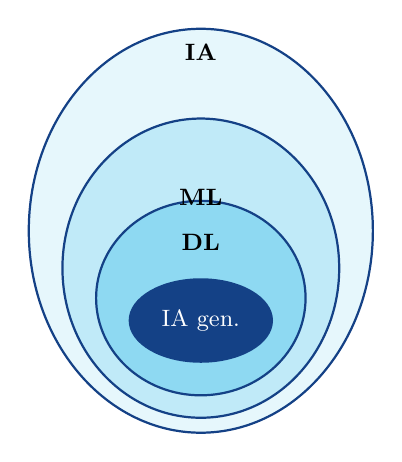
\begin{tikzpicture}[scale=0.95, transform shape,
	lvl/.style={ellipse, draw=UCMNavy, thick, align=center, font=\small}]
	\node[lvl, fill=UCMBlue!10, minimum width=4.6cm, minimum height=5.4cm] (ai) at (0,0) {};
	\node[lvl, fill=UCMBlue!25, minimum width=3.7cm, minimum height=4.0cm] (ml) at (0,-0.5) {};
	\node[lvl, fill=UCMBlue!45, minimum width=2.8cm, minimum height=2.6cm] (dl) at (0,-0.9) {};
	\node[lvl, fill=UCMNavy, text=white, minimum width=1.9cm, minimum height=1.1cm] (gen) at (0,-1.2) {IA gen.};
	\node[font=\small, above=0.05cm of ai.center, yshift=2.1cm] {\textbf{IA}};
	\node[font=\small, yshift=0.95cm] at (ml.center) {\textbf{ML}};
	\node[font=\small, yshift=0.75cm] at (dl.center) {\textbf{DL}};
\end{tikzpicture}
\end{center}
\end{column}
\end{columns}
\vspace{0.3em}
\footnotesize Toda la IA generativa es aprendizaje profundo, pero \textbf{no} toda la IA es aprendizaje autom\'atico.
\end{frame}

\begin{frame}
\frametitle{IA estrecha vs. IA general (AGI)}
\begin{columns}[T]
\begin{column}{6cm}
\begin{block}{IA estrecha (\emph{narrow})}
\begin{itemize}
	\item Es toda la IA que existe hoy.
	\item Entrenada para una \textbf{familia acotada} de tareas.
	\item Reconocimiento facial, traducci\'on, recomendaci\'on, asistentes.
	\item Rendimiento sobrehumano en algunas tareas y fr\'agil fuera de su dominio.
\end{itemize}
\end{block}
\end{column}
\begin{column}{6cm}
\begin{alertblock}{IA general (AGI)}
\begin{itemize}
	\item Competencia amplia al nivel humano en \textbf{tareas nuevas}.
	\item No existe una definici\'on operativa aceptada, ni una prueba consensuada.
	\item Cuidado: los modelos actuales combinan capacidad muy alta con fallos elementales (lo veremos con datos).
\end{itemize}
\end{alertblock}
\end{column}
\end{columns}
\vspace{0.4em}
\begin{center}

\begin{tikzpicture}[font=\small]
	\node[rectangle, draw=UCMNavy, thick, rounded corners, fill=UCMBlue!20, minimum width=3.2cm, minimum height=0.75cm] (n) at (0,0) {IA estrecha};
	\node[rectangle, draw=StanfordRed, thick, rounded corners, fill=StanfordRed!12, minimum width=3.2cm, minimum height=0.75cm] (g) at (7,0) {AGI};
	\draw[<->, very thick, UCMNavy] (n) -- (g) node[midway, above, font=\scriptsize] {generalizaci\'on a tareas no vistas};
\end{tikzpicture}
\end{center}
\end{frame}

\begin{frame}
\frametitle{La prueba de Turing: ¿pueden pensar las máquinas?}
\begin{columns}[T]
\begin{column}{6.2cm}
Propuesta por Alan Turing en 1950 como sustituto \emph{operacional} de una pregunta que consideraba mal planteada.
\begin{block}{El juego de la imitación}
Un interrogador humano (C) conversa por texto con un humano (B) y una m\'aquina (A). Si C no logra distinguir de forma consistente qui\'en es qui\'en, la m\'aquina supera la prueba.
\end{block}
\onslide<2->{%
\footnotesize
\textbf{Crítica moderna:} mide la capacidad de \emph{imitar}, no de razonar. Por eso hoy se eval\'ua con \emph{benchmarks} de tareas concretas y con comparaciones ciegas entre modelos (\emph{arenas}).}
\end{column}
\begin{column}{5.8cm}
\begin{center}
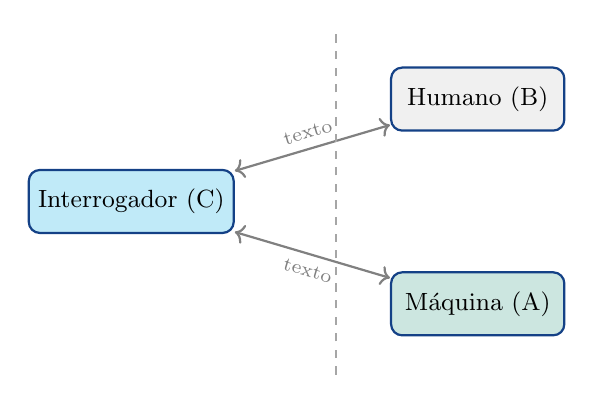
\begin{tikzpicture}[font=\small,
	caja/.style={rectangle, draw=UCMNavy, thick, rounded corners, fill=LightGray, minimum height=0.8cm, minimum width=2.2cm}]
	\node[caja, fill=UCMBlue!25] (c) at (0,0) {Interrogador (C)};
	\node[caja] (b) at (4.4,1.3) {Humano (B)};
	\node[caja, fill=AccentGreen!20] (a) at (4.4,-1.3) {M\'aquina (A)};
	\draw[<->, thick, gray] (c) -- (b) node[midway, above, sloped, font=\scriptsize] {texto};
	\draw[<->, thick, gray] (c) -- (a) node[midway, below, sloped, font=\scriptsize] {texto};
	\draw[dashed, gray!70] (2.6,-2.2) -- (2.6,2.2);
\end{tikzpicture}
\end{center}
\end{column}
\end{columns}
\end{frame}

%=====================================================================
\section{Una breve historia}
%=====================================================================

\begin{frame}
\frametitle{Setenta años en una lámina}
\begin{center}
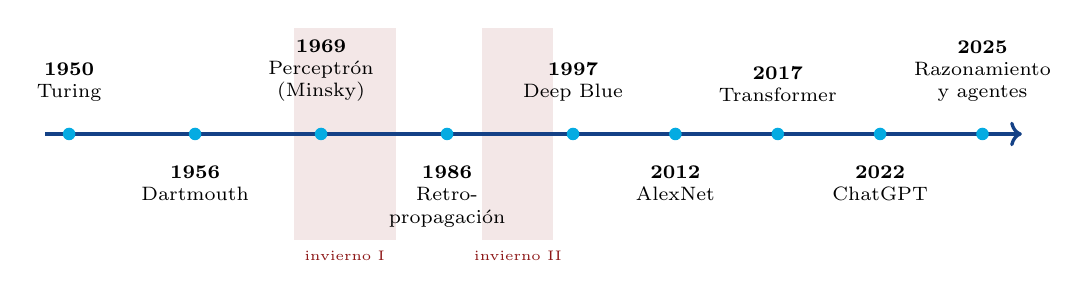
\begin{tikzpicture}[font=\scriptsize, hito/.style={circle, fill=UCMBlue, inner sep=1.6pt}]
	\draw[->, very thick, UCMNavy] (0,0) -- (12.4,0);
	\foreach \x/\a/\t [count=\i] in {
		0.3/1950/Turing,
		1.9/1956/Dartmouth,
		3.5/1969/{Perceptrón\\(Minsky)},
		5.1/1986/{Retro-\\propagación},
		6.7/1997/{Deep Blue},
		8.0/2012/{AlexNet},
		9.3/2017/{Transformer},
		10.6/2022/{ChatGPT},
		11.9/2025/{Razonamiento\\y agentes}}{
		\node[hito] (h\i) at (\x,0) {};
		\ifodd\i
			\node[above=2mm of h\i, align=center, font=\scriptsize] {\textbf{\a}\\\t};
		\else
			\node[below=2mm of h\i, align=center, font=\scriptsize] {\textbf{\a}\\\t};
		\fi
	}
	\begin{scope}[on background layer]
		\fill[StanfordRed, opacity=0.10] (3.15,-1.35) rectangle (4.45,1.35);
		\fill[StanfordRed, opacity=0.10] (5.55,-1.35) rectangle (6.45,1.35);
	\end{scope}
	\node[StanfordRed, font=\tiny] at (3.80,-1.55) {invierno I};
	\node[StanfordRed, font=\tiny] at (6.00,-1.55) {invierno II};
\end{tikzpicture}
\end{center}
\vspace{0.6em}
\begin{itemize}
	\item El campo avanza \textbf{a saltos}: cada ola nace de una idea algor\'itmica que se vuelve viable gracias al hardware y a los datos disponibles.
	\item Las dos \'ultimas d\'ecadas son la excepci\'on: crecimiento sostenido, sin invierno intermedio.
\end{itemize}
\end{frame}

\begin{frame}
\frametitle{Los inviernos de la IA}
\begin{columns}[T]
\begin{column}{6cm}
\begin{exampleblock}{Épocas de optimismo}
\begin{itemize}
	\item \textbf{1950--70:} fundaci\'on, l\'ogica simb\'olica y grandes promesas.
	\item \textbf{1980s:} auge industrial de los sistemas expertos.
	\item \textbf{2012--hoy:} datos masivos, GPUs y aprendizaje profundo.
\end{itemize}
\end{exampleblock}
\end{column}
\begin{column}{6cm}
\begin{alertblock}{Los inviernos}
\begin{itemize}
	\item \textbf{1974--80} y \textbf{1987--93}: recortes de financiamiento y p\'erdida de inter\'es.
	\item Causas: promesas excesivas, l\'imites de c\'omputo y de datos, costo de mantener sistemas basados en reglas.
\end{itemize}
\end{alertblock}
\end{column}
\end{columns}
\vspace{0.5em}
\begin{block}{Lección para este curso}
Distinguir siempre entre lo que un sistema \textbf{demuestra} en una evaluaci\'on y lo que se \textbf{afirma} sobre \'el. Gran parte de esta clase consiste en aprender a leer evidencia.
\end{block}
\end{frame}

\begin{frame}
\frametitle{¿Qué cambió en la última década?}
\begin{columns}[T]
\begin{column}{4cm}
\begin{block}{Datos}
De miles a \textbf{decenas de billones} de tokens de entrenamiento. La web como corpus.
\end{block}
\end{column}
\begin{column}{4cm}
\begin{block}{Cómputo}
GPUs y aceleradores dedicados; \'ordenes de magnitud m\'as de c\'omputo por modelo.
\end{block}
\end{column}
\begin{column}{4cm}
\begin{block}{Algoritmos}
Retropropagaci\'on a escala, \emph{transformers}, aprendizaje auto-supervisado y por refuerzo.
\end{block}
\end{column}
\end{columns}
\vspace{0.8em}
\pause
\begin{itemize}
	\item Ninguno de los tres factores basta por s\'i solo: el \emph{transformer} (2017) es un algoritmo, pero solo rinde con datos y c\'omputo a escala.
	\item Consecuencia econ\'omica: en 2025, la \textbf{industria} produjo m\'as del 90\% de los modelos notables, y los m\'as capaces son tambi\'en los menos transparentes.
\end{itemize}
\end{frame}

%=====================================================================
\section{Dos paradigmas: símbolos y conexiones}
%=====================================================================

\begin{frame}
\frametitle{Símbolos vs. conexiones}
\begin{columns}[T]
\begin{column}{6cm}
\begin{block}{IA simbólica (\emph{top-down})}
\begin{itemize}
	\item \textbf{Idea:} la inteligencia surge de manipular s\'imbolos con reglas l\'ogicas.
	\item \textbf{M\'etodo:} representar el conocimiento expl\'icitamente y aplicar un motor de inferencia.
	\item \textbf{Ejemplo:} \texttt{SI fiebre > 38 Y tos = seca ENTONCES gripe}
	\item[+] Transparente y auditable.
	\item[--] Cuesta capturar el conocimiento; fr\'agil ante lo no previsto.
\end{itemize}
\end{block}
\end{column}
\begin{column}{6cm}
\begin{block}{IA conexionista (\emph{bottom-up})}
\begin{itemize}
	\item \textbf{Idea:} la inteligencia emerge de la interacci\'on de muchas unidades simples.
	\item \textbf{M\'etodo:} aprender patrones y representaciones directamente de los datos.
	\item \textbf{Ejemplo:} redes neuronales profundas.
	\item[+] Escala con datos y c\'omputo; no requiere reglas.
	\item[--] Opaca; depende de la calidad de los datos.
\end{itemize}
\end{block}
\end{column}
\end{columns}
\vspace{0.4em}
\pause
\footnotesize
\textbf{Hoy la frontera se difumina:} los sistemas de producci\'on combinan un modelo neuronal con estructuras simb\'olicas externas (llamadas a herramientas, bases de datos, verificadores, restricciones formales).
\end{frame}

%=====================================================================
\section{Aprendizaje automático}
%=====================================================================

\begin{frame}
\frametitle{El ciclo del aprendizaje automático}
\begin{center}
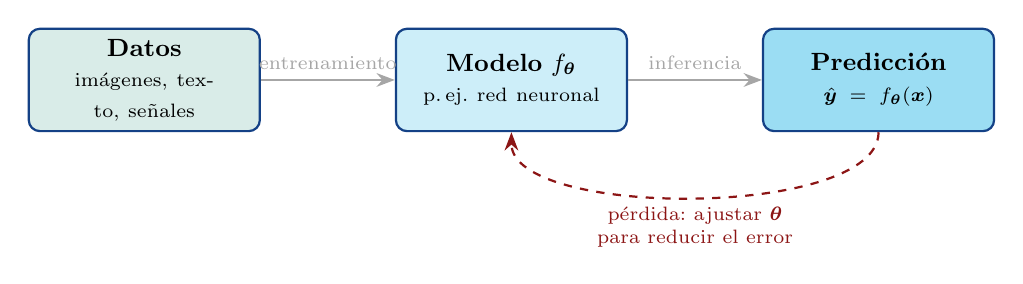
\begin{tikzpicture}[font=\small, node distance=1.2cm,
	caja/.style={rectangle, draw=UCMNavy, thick, rounded corners, align=center,
		text width=2.7cm, minimum height=1.3cm},
	flecha/.style={->, >=Stealth, thick, gray!70}]
	\node[caja, fill=AccentGreen!15] (datos) at (0,0) {\textbf{Datos}\\{\scriptsize im\'agenes, texto, se\~nales}};
	\node[caja, fill=UCMBlue!20, right=1.7cm of datos] (modelo) {\textbf{Modelo} $f_{\bm\theta}$\\{\scriptsize p.\,ej. red neuronal}};
	\node[caja, fill=UCMBlue!40, right=1.7cm of modelo] (pred) {\textbf{Predicci\'on}\\{\scriptsize $\hat{\y}=f_{\bm\theta}(\x)$}};
	\draw[flecha] (datos) -- (modelo) node[midway, above, font=\scriptsize] {entrenamiento};
	\draw[flecha] (modelo) -- (pred) node[midway, above, font=\scriptsize] {inferencia};
	\draw[flecha, dashed, StanfordRed] (pred.south) .. controls +(down:1.1cm) and +(down:1.1cm) .. (modelo.south)
		node[midway, below, align=center, font=\scriptsize, StanfordRed] {p\'erdida: ajustar $\bm\theta$\\para reducir el error};
\end{tikzpicture}
\end{center}
\vspace{0.6em}
\begin{itemize}
	\item El programador ya no escribe la regla: escribe el \textbf{objetivo} (la funci\'on de p\'erdida) y deja que la optimizaci\'on encuentre los par\'ametros.
	\item Todo el resto del curso son variaciones sobre este ciclo.
\end{itemize}
\end{frame}

\begin{frame}
\frametitle{La misma idea, en tres líneas de matemática}
Dado un conjunto de datos $\mathcal{D}=\{(\x_i,\y_i)\}_{i=1}^{n}$ y una familia de funciones $f_{\bm\theta}$ con par\'ametros $\bm\theta$:
\formula{
\[
\bm\theta^{\star} \;=\; \arg\min_{\bm\theta}\; \underbrace{\frac{1}{n}\sum_{i=1}^{n} \ell\big(f_{\bm\theta}(\x_i),\, \y_i\big)}_{\text{error en los datos}} \;+\; \underbrace{\lambda\, \Omega(\bm\theta)}_{\text{regularizaci\'on}}
\]}
\pause
\begin{itemize}
	\item $\ell$ es la \textbf{funci\'on de p\'erdida}: define qu\'e significa equivocarse (clase 1.5).
	\item $\Omega$ penaliza soluciones complejas y controla el \textbf{sobreajuste} (clase 1.4).
	\item El $\arg\min$ se resuelve por \textbf{descenso de gradiente} (clase 1.6).
	\pause
	\item Lo que interesa no es el error en $\mathcal{D}$, sino el error esperado en datos nuevos:
	\[ \E_{(\x,\y)\sim P}\big[\ell(f_{\bm\theta}(\x),\y)\big] \quad\text{---\; el problema de la \textbf{generalizaci\'on}.} \]
\end{itemize}
\end{frame}

\begin{frame}
\frametitle{Cuatro paradigmas de aprendizaje}
\begin{columns}[T]
\begin{column}{6cm}
\begin{block}{Supervisado}
Aprender de pares (entrada, \textbf{etiqueta}).\\
{\scriptsize Diagn\'ostico a partir de im\'agenes m\'edicas etiquetadas.}
\end{block}
\begin{block}{No supervisado}
Encontrar estructura \textbf{sin} etiquetas.\\
{\scriptsize Segmentar clientes por comportamiento de compra.}
\end{block}
\end{column}
\begin{column}{6cm}
\begin{block}{Auto-supervisado}
La etiqueta se \textbf{extrae de los propios datos}: predecir la palabra siguiente, reconstruir una parte oculta.\\
{\scriptsize Es lo que hace posible entrenar un LLM sobre texto no etiquetado.}
\end{block}
\begin{block}{Por refuerzo}
Aprender por \textbf{ensayo y error} maximizando una recompensa.\\
{\scriptsize Control, juegos y ajuste de modelos de lenguaje por preferencias.}
\end{block}
\end{column}
\end{columns}
\vspace{0.4em}
\footnotesize Los sistemas actuales encadenan varios: pre-entrenamiento auto-supervisado $\rightarrow$ ajuste supervisado $\rightarrow$ refuerzo con retroalimentaci\'on.
\end{frame}

\begin{frame}
\frametitle{El ecosistema de la IA}
\begin{center}
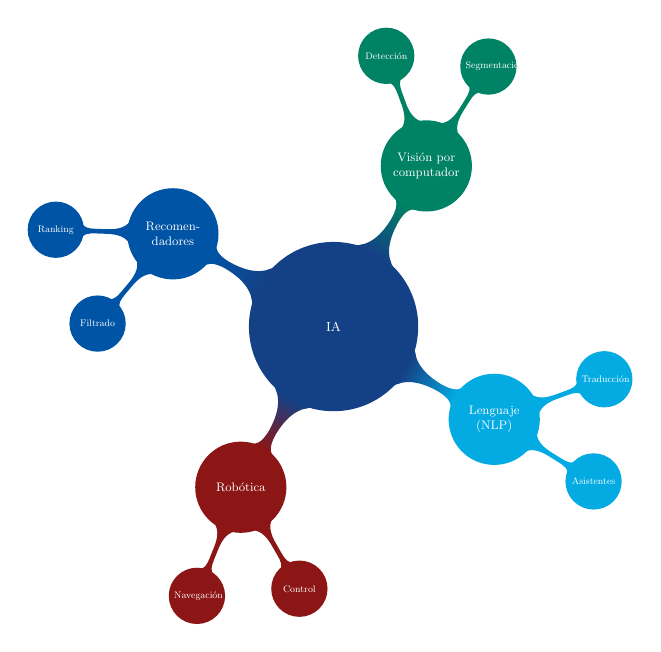
\begin{tikzpicture}[scale=0.62, transform shape]
	\path[mindmap, concept color=UCMNavy, text=white,
		every node/.style={concept, font=\small},
		level 1 concept/.append style={level distance=38mm, sibling angle=90},
		level 2 concept/.append style={level distance=24mm, sibling angle=52}]
	node[concept, scale=0.85] {IA}
	[clockwise from=60]
	child[concept color=AccentGreen] {
		node[concept, scale=0.8] {Visi\'on por computador}
		[clockwise from=110]
		child { node[concept, scale=0.62] {Detecci\'on} }
		child { node[concept, scale=0.62] {Segmentaci\'on} }
	}
	child[concept color=UCMBlue] {
		node[concept, scale=0.8] {Lenguaje (NLP)}
		[clockwise from=20]
		child { node[concept, scale=0.62] {Traducci\'on} }
		child { node[concept, scale=0.62] {Asistentes} }
	}
	child[concept color=StanfordRed] {
		node[concept, scale=0.8] {Rob\'otica}
		[clockwise from=-60]
		child { node[concept, scale=0.62] {Control} }
		child { node[concept, scale=0.62] {Navegaci\'on} }
	}
	child[concept color=AccentBlue] {
		node[concept, scale=0.8] {Recomen-\\dadores}
		[clockwise from=-130]
		child { node[concept, scale=0.62] {Filtrado} }
		child { node[concept, scale=0.62] {Ranking} }
	};
\end{tikzpicture}
\end{center}
\end{frame}

%=====================================================================
\section{El estado del arte: AI Index 2026}
%=====================================================================

\begin{frame}
\frametitle{AI Index 2026: seis conclusiones}
\footnotesize
\begin{enumerate}
	\item \textbf{La capacidad no se est\'a estancando.} La industria produjo m\'as del 90\% de los modelos frontera de 2025, y varios superan la l\'inea base humana en preguntas cient\'ificas de nivel doctoral y en matem\'atica de competencia.
	\pause
	\item \textbf{La brecha EE.UU.--China se cerr\'o.} Los mejores modelos de ambos pa\'ises se han alternado el liderazgo desde 2025; en marzo de 2026 la diferencia es de 2{,}7\%.
	\pause
	\item \textbf{La frontera es irregular (\emph{jagged}).} Los mismos modelos que ganan medalla de oro en la Olimpiada Internacional de Matem\'atica fallan al leer un reloj anal\'ogico.
	\pause
	\item \textbf{La IA responsable no sigue el ritmo.} Los incidentes documentados subieron a \textbf{362} en 2025 (233 en 2024).
	\pause
	\item \textbf{La adopci\'on es hist\'oricamente r\'apida.} La IA generativa alcanz\'o $\approx$53\% de adopci\'on poblacional en tres a\~nos; 88\% de las organizaciones la usan.
	\pause
	\item \textbf{La huella ambiental crece con las capacidades.} El entrenamiento de Grok 4 emiti\'o 72.816 toneladas de CO$_2$ equivalente.
\end{enumerate}
\vspace{0.3em}
{\scriptsize\color{StanfordGray} Fuente: \emph{AI Index Report 2026}, Stanford HAI --- \emph{Top Takeaways}.
\url{https://hai.stanford.edu/ai-index/2026-ai-index-report}}
\end{frame}

\begin{frame}
\frametitle{Escala: parámetros de los modelos notables}
\figai{ai2026_parametros}{0.64}
\lectura{El crecimiento en par\'ametros reportados se aplana despu\'es de 2022, pero en gran medida porque los laboratorios frontera \textbf{dejaron de publicar} el dato. Ausencia de evidencia no es evidencia de ausencia.}
\fuenteai{1.1.10}
\end{frame}

\begin{frame}
\frametitle{Datos: tamaño del conjunto de entrenamiento}
\figai{ai2026_datos}{0.64}
\lectura{Escala logar\'itmica: en quince a\~nos el corpus de entrenamiento pas\'o de $10^4$ a m\'as de $10^{13}$ tokens. El cuello de botella se desplaza desde el algoritmo hacia los datos.}
\fuenteai{1.1.11}
\end{frame}

\begin{frame}
\frametitle{Rendimiento frente a la línea base humana}
\figai{ai2026_benchmarks}{0.64}
\lectura{Cada curva es un \emph{benchmark} normalizado al 100\,\% humano. El patr\'on se repite: a\~nos de avance lento, luego saturaci\'on en pocos meses. Por eso los \emph{benchmarks} caducan.}
\fuenteai{2.1.1}
\end{frame}

\begin{frame}
\frametitle{Comprensión del lenguaje: MMLU-Pro}
\figai{ai2026_mmlu}{0.64}
\lectura{Los quince mejores modelos se agrupan entre 87\,\% y 91\,\%: la prueba ya casi no discrimina. Cuando un \emph{benchmark} se satura, deja de informar y hay que reemplazarlo.}
\fuenteai{2.2.1}
\end{frame}

\begin{frame}
\frametitle{Matemática: cuando el problema es realmente difícil}
\begin{columns}[T]
\begin{column}{6.2cm}
\begin{itemize}[<+->]
	\item \textbf{MathArena} (problemas de competencia reci\'en publicados): la exactitud subi\'o de $\approx$83\,\% a \textbf{97\,\%} entre noviembre y diciembre de 2025.
	\item \textbf{FrontierMath Tier 4} (problemas originales que a un matem\'atico profesional le toman horas o d\'ias): de casi 0\,\% a \textbf{31,3\,\%}.
	\item Misma capacidad, dos lecturas opuestas seg\'un la dificultad del instrumento.
\end{itemize}
\vspace{0.4em}
\begin{block}<3->{Implicación metodológica}
Al leer un resultado, la primera pregunta no es \emph{cu\'anto} sac\'o el modelo, sino \textbf{qu\'e mide la prueba} y si sus \'items pudieron estar en el entrenamiento (\emph{contaminaci\'on}).
\end{block}
\end{column}
\begin{column}{5.8cm}
\begin{center}
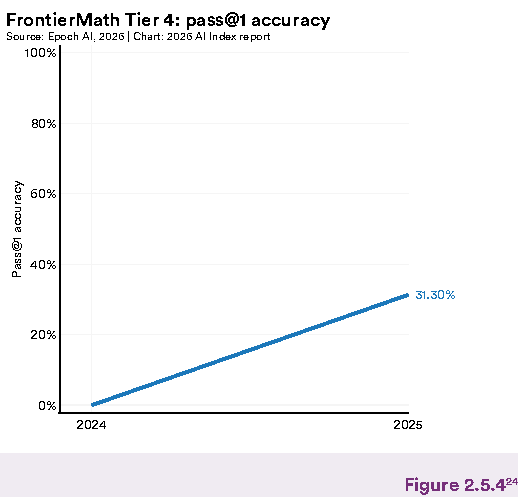
\includegraphics[width=\linewidth, height=0.6\textheight, keepaspectratio]{figures/ai2026_frontiermath}
\end{center}
\end{column}
\end{columns}
\vspace{0.2em}
\fuenteai{2.5.4 y 2.5.5}
\end{frame}

\begin{frame}
\frametitle{Razonamiento abstracto: ARC-AGI-2}
\figai{ai2026_arcagi2}{0.64}
\lectura{ARC-AGI-2 mide inferencia de reglas a partir de unos pocos ejemplos. El mejor modelo llega a 84,6\,\%, con una dispersi\'on de casi 46 puntos entre modelos: la capacidad de \emph{generalizar} var\'ia mucho m\'as que la de \emph{recordar}.}
\fuenteai{2.4.3}
\end{frame}

\begin{frame}
\frametitle{La frontera irregular: leer un reloj}
\figai{ai2026_clockbench}{0.64}
\lectura{El mejor modelo lee correctamente un reloj anal\'ogico el \textbf{50,6\,\%} de las veces, frente a $\approx$90\,\% de las personas. La misma familia de modelos gana medalla de oro en la Olimpiada Internacional de Matem\'atica.}
\fuenteai{2.4.8}
\end{frame}

\begin{frame}
\frametitle{Ingeniería de software: SWE-bench}
\figai{ai2026_swebench}{0.64}
\lectura{SWE-bench eval\'ua la resoluci\'on de \emph{issues} reales de GitHub. En un a\~no el rendimiento pas\'o del 60\,\% al $\approx$100\,\% de la l\'inea base humana. Terminal-Bench 2.0 subi\'o de 20\,\% a 77,3\,\% en el mismo per\'iodo.}
\fuenteai{2.5.1}
\end{frame}

\begin{frame}
\frametitle{Agentes: sistemas que ejecutan tareas de varios pasos}
\begin{columns}[T]
\begin{column}{6.4cm}
\begin{center}
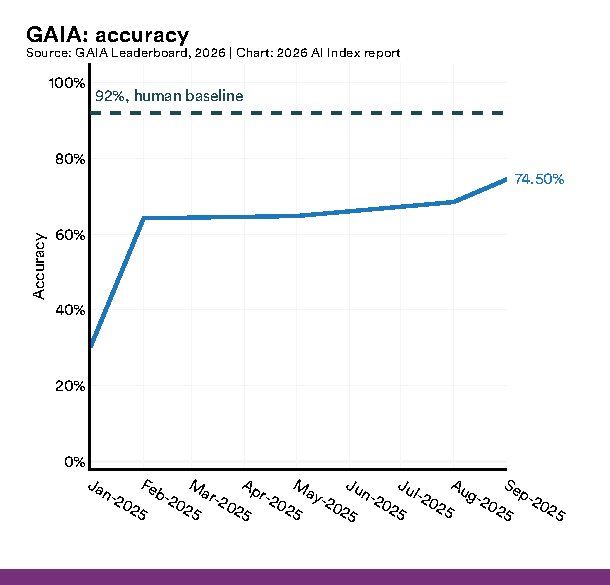
\includegraphics[width=\linewidth, height=0.58\textheight, keepaspectratio]{figures/ai2026_gaia}
\end{center}
\end{column}
\begin{column}{5.6cm}
\begin{itemize}
	\item Un \textbf{agente} no responde: navega, llama herramientas, manipula archivos y encadena pasos hasta cumplir un objetivo.
	\item \textbf{GAIA:} de $\approx$20\,\% (enero 2025) a \textbf{74,5\,\%}, frente a 92\,\% humano.
	\item \textbf{OSWorld} (tareas reales de escritorio): de 12\,\% a $\approx$66\,\%.
	\pause
	\item Pero a\'un fallan \textbf{1 de cada 3} intentos en pruebas estructuradas: suficiente para asistir, insuficiente para delegar sin supervisi\'on.
\end{itemize}
\end{column}
\end{columns}
\vspace{0.2em}
\fuenteai{2.6.1}
\end{frame}

\begin{frame}
\frametitle{Geopolítica del rendimiento: EE.UU. vs. China}
\figai{ai2026_arena_us_china}{0.64}
\lectura{La ventaja estadounidense de 2023 pr\'acticamente desapareci\'o: 39 puntos Elo (2,7\,\%) en marzo de 2026. En inversi\'on privada, en cambio, la asimetr\'ia persiste: 285,9 mil millones de d\'olares en EE.UU.\ frente a 12,4 mil millones en China.}
\fuenteai{2.1.3}
\end{frame}

\begin{frame}
\frametitle{Adopción: más rápida que el PC y que internet}
\figai{ai2026_adopcion}{0.64}
\lectura{Medido desde el primer producto masivo de cada tecnolog\'ia, la IA generativa lleg\'o al 53\,\% de la poblaci\'on en tres a\~nos. La adopci\'on correlaciona fuertemente con el PIB per c\'apita.}
\fuenteai{4.3.9}
\end{frame}

%=====================================================================
\section{Riesgos, ética y sostenibilidad}
%=====================================================================

\begin{frame}
\frametitle{Cuatro problemas que no son técnicos (solamente)}
\begin{columns}[T]
\begin{column}{6cm}
\begin{alertblock}{Sesgo}
El modelo aprende los sesgos de sus datos y los aplica a escala.\\
{\scriptsize Selecci\'on de personal, cr\'edito, reconocimiento facial.}
\end{alertblock}
\begin{block}{Transparencia y explicabilidad}
¿Por qu\'e el modelo decidi\'o esto?\\
{\scriptsize Cr\'itico en medicina, finanzas y justicia; los modelos m\'as capaces son los m\'as opacos.}
\end{block}
\end{column}
\begin{column}{6cm}
\begin{block}{Privacidad}
Los modelos pueden memorizar y filtrar datos sensibles del entrenamiento.\\
{\scriptsize Riesgo agravado cuando se ajustan con datos internos.}
\end{block}
\begin{block}{Responsabilidad}
¿Qui\'en responde ante un da\~no: quien desarrolla, quien despliega o quien usa?\\
{\scriptsize La respuesta es regulatoria, no algor\'itmica.}
\end{block}
\end{column}
\end{columns}
\vspace{0.4em}
\footnotesize Los desarrolladores frontera reportan casi siempre m\'etricas de capacidad, pero el reporte de \emph{benchmarks} de IA responsable sigue siendo irregular.
\end{frame}

\begin{frame}
\frametitle{Incidentes documentados}
\figai{ai2026_incidentes}{0.64}
\lectura{362 incidentes en 2025 frente a 233 en 2024. Parte del alza es mayor cobertura y mejor registro; aun as\'i, la tendencia acompa\~na a la adopci\'on, no a la madurez de las salvaguardas.}
\fuenteai{3.2.1}
\end{frame}

\begin{frame}
\frametitle{Huella ambiental del entrenamiento}
\figai{ai2026_carbono}{0.64}
\lectura{De 0,01 toneladas de CO$_2$e (AlexNet, 2012) a \textbf{72.816} (Grok 4, 2025). Adem\'as, la capacidad el\'ectrica de los centros de datos de IA lleg\'o a 29,6 GW, comparable al consumo peak del estado de Nueva York.}
\fuenteai{1.4.3}
\end{frame}

\begin{frame}
\frametitle{¿Y desde Chile?}
\begin{columns}[T]
\begin{column}{6cm}
\begin{block}{Producción de modelos}
Am\'erica Latina y el Caribe registran solo \textbf{2} modelos notables acumulados, frente a 666 de Europa y Asia Central. La regi\'on impulsa iniciativas propias como \textbf{Latam-GPT}.
\end{block}
\end{column}
\begin{column}{6cm}
\begin{exampleblock}{Habilidades}
Chile aparece, junto con Emiratos \'Arabes Unidos y Sud\'africa, entre los pa\'ises con \textbf{crecimiento m\'as r\'apido en habilidades de ingenier\'ia de IA}, no solo de alfabetizaci\'on digital.
\end{exampleblock}
\end{column}
\end{columns}
\vspace{0.6em}
\begin{block}{Consecuencia para ustedes}
La ventaja competitiva local no est\'a en entrenar modelos frontera, sino en \textbf{adaptarlos y evaluarlos} sobre problemas y datos propios. Eso exige entender el ciclo completo: datos, p\'erdida, optimizaci\'on y evaluaci\'on.
\end{block}
\vspace{0.2em}
\fuenteai{cap\'itulos 1 y 7}
\end{frame}

%=====================================================================
\section{Cierre}
%=====================================================================

\begin{frame}
\frametitle{Resumen}
\begin{center}
\begin{tabular}{ll}
\toprule
\textbf{Concepto} & \textbf{Idea clave}\\
\midrule
IA                & Agentes que perciben, razonan y act\'uan racionalmente\\
IA / ML / DL      & Subconjuntos anidados; no toda la IA aprende de datos\\
Paradigmas        & S\'imbolos (reglas) vs.\ conexiones (datos); hoy, h\'ibridos\\
Ciclo de ML       & Datos $\rightarrow$ p\'erdida $\rightarrow$ optimizaci\'on $\rightarrow$ generalizaci\'on\\
Estado del arte   & Capacidad alt\'isima pero \textbf{irregular}: la frontera es dentada\\
Evaluaci\'on      & Los \emph{benchmarks} se saturan; hay que leerlos con criterio\\
Riesgos           & Sesgo, opacidad, privacidad, responsabilidad, energ\'ia\\
\bottomrule
\end{tabular}
\end{center}
\vspace{0.8em}
\begin{itemize}
	\item La pregunta \'util no es ``¿la IA puede hacer X?'', sino \textbf{``¿bajo qu\'e evaluaci\'on, con qu\'e datos y con qu\'e tasa de error?''}
	\item En la pr\'oxima clase abrimos la caja: sistemas expertos, el paradigma simb\'olico en detalle.
\end{itemize}
\end{frame}

\begin{frame}
\frametitle{Para profundizar}
\begin{itemize}
	\item Stanford HAI, \emph{AI Index Report 2026}\\ \url{https://hai.stanford.edu/ai-index/2026-ai-index-report}
	\item Russell \& Norvig, \emph{Artificial Intelligence: A Modern Approach}, cap.~1--2.
	\item Prince, \emph{Understanding Deep Learning} (libro abierto)\\ \url{https://udlbook.github.io/udlbook/}
	\item Zhang, Lipton, Li \& Smola, \emph{Dive into Deep Learning}\\ \url{https://d2l.ai/}
	\item Turing (1950), \emph{Computing Machinery and Intelligence}, \emph{Mind}.
	\item Bommasani et al.\ (2021), \emph{On the Opportunities and Risks of Foundation Models}.
\end{itemize}
\vspace{0.8em}
\begin{center}
\Large \textbf{¿Preguntas?}
\end{center}
\end{frame}

\end{document}
